\section{Integrazione numerica}

\subsection{Introduzione}

Alcuni problemi ingegneristici richiedono il calcolo di integrali, talvolta pure molto complessi. Non sempre si riesce a trovare in forma esplicita la primitiva di una funzione, anche nel caso in cui la si conosca, potrebbe essere difficile valutarla (come ad esempio $f\left(x\right) = \cos\left(4x\right) \cos\left(3\sin\left(x\right)\right)$).

\highspace
In tutti questi casi, è necessario utilizzare metodi numerici in gradi di restituire un valore approssimato della quantità di interesse, indipendentemente da quanto complessa sia la funzione da integrare o da differenziare. In questo capitolo, vengono presentati alcuni metodi per l'\textbf{approssimazione numerica di integrali di funzioni}, i quali vengono chiamate \definition{formule di quadratura}.

\highspace
\begin{flushleft}
	\textcolor{Green3}{\faIcon{book} \textbf{Alcune notazioni e definizioni di introduzione}}
\end{flushleft}
Si consideri l'integrale:
\begin{equation}\label{eq: formula di quadratura base}
	I\left(f\right) = \int_{a}^{b} f\left(x\right) \:\mathrm{d}x
\end{equation}
Si suddivida l'intervallo $\left[a,b\right]$ in $M$ intervalli $I_{k}$ di ampiezza costante $H$:
\begin{equation*}
	\left[x_{k-1}, x_{k}\right] \hspace{1em} k = 1, \dots, M \hspace{3em}
	x_{k} = a + kH \hspace{1em} k = 0, \dots, M
\end{equation*}
Si introduce inoltre su ogni intervallo i punti medi:
\begin{equation*}
	\overline{x}_{k} = \dfrac{x_{k-1} + x_{k}}{2}
\end{equation*}
\begin{figure}[!htp]
	\centering
	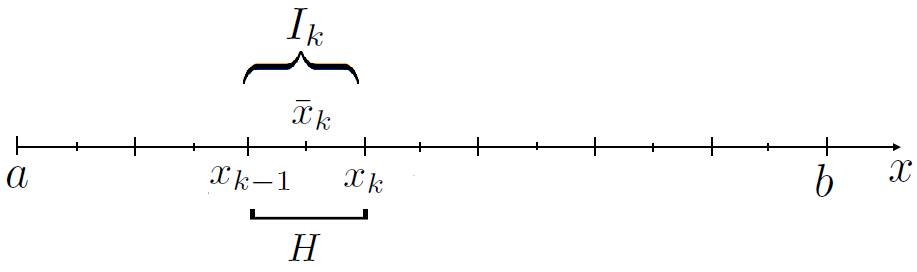
\includegraphics[width=0.6\textwidth]{img/formule-di-quadratura-1.png}
\end{figure}

\highspace
Si consideri una \textbf{formula di quadratura} per il calcolo approssimato dell'integrale nell'equazione \ref{eq: formula di quadratura base} e sia $I_{H}\left(f\right)$ il valore approssimato ottenuto.

La \textbf{formula di quadratura} è di \textbf{ordine $p$} se l'\emph{errore} soddisfa la seguente stima:
\begin{equation}
	E_{H} = \left|I\left(f\right) - I_{H}\left(f\right)\right| \le CH^{p}
\end{equation}
Inoltre, la formula di quadratura ha \textbf{grado di esattezza pari ad $r$} se essa risulta esatta quando applicata \textbf{ai polinomi di grado minore o uguale ad $r$}, ovverosia se:
\begin{equation}
	E_{H} = \left|I\left(f\right) - I_{H}\left(f\right)\right| = 0 \hspace{2em} \forall f \in \mathbb{P}^{r} \left(a,b\right)
\end{equation}